\subsection{Belbin Test}
A Belbin test, is a test of a lot of questionares, filled out by the person the test is about, and by previous group members of this person. This means that there is both self perception and how other people see the person. It is focused around how a person acts and works in a group. Each person in the group takes the test, and from that, is it seen which roles should be taken from which group member. It is a tool, that should make sure the process of making a project runs as smoothly as possible. 
\begin{figure} [h!]
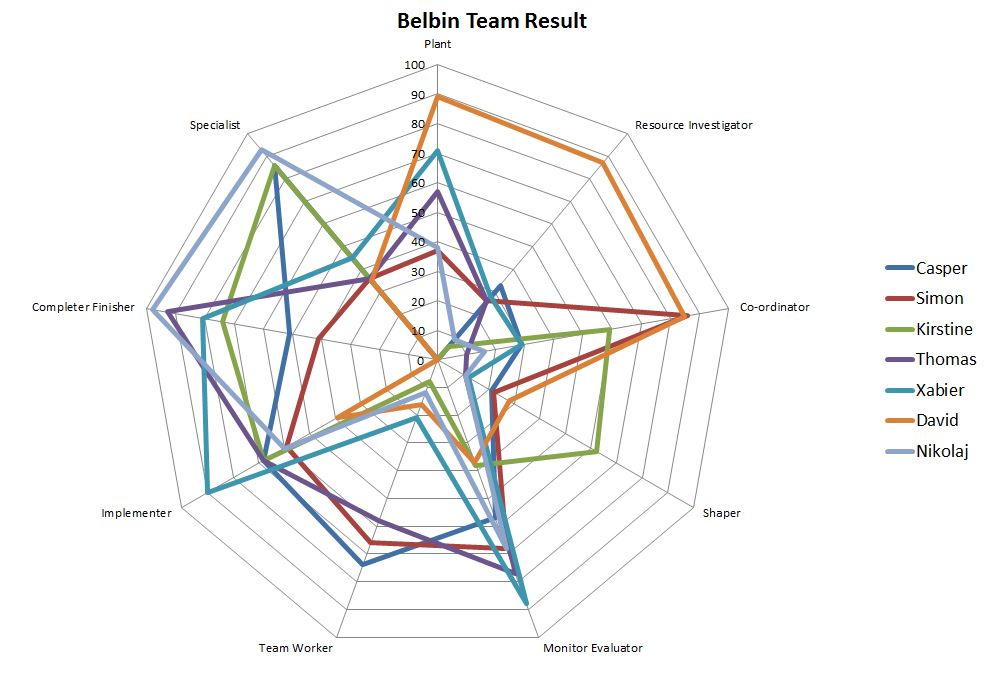
\includegraphics[width=\textwidth]{./graphics/Belbin_spiderweb}
\caption{Belbin Self-perception "Spiderweb". Each person has a color, and on the axis is how much we see our selves is the given role, as a percentage.}
\label{belbinspider}
\end{figure}

\begin{table}[ht]
\centering
\begin{tabular}{|p{0.45\textwidth}|p{0.45\textwidth}|}
\hline
\multicolumn{1}{|c|}{\textit{Contribution:}}                                                      & \multicolumn{1}{c|}{\textit{Allowable Weaknesses:}}                          \\ \hline
\multicolumn{2}{|l|}{\textbf{Top 3 roles:}}                                                                                                                                      \\ \hline
\multicolumn{2}{|c|}{\textbf{Monitor Evaluator}}                                                                                                                                 \\ \hline
Sober, strategic and discerning. Sees all options and judges accurately.                          & Lacks drive and ability to inspire others. Can be overly critical to others. \\ \hline
\multicolumn{2}{|c|}{\textbf{Implementer}}                                                                                                                                       \\ \hline
Practical, reliable, efficient. Turns ideas into actions and organizes work that needs to be done.& Somewhat inflexible. Slow to respond to new possibilities.                   \\ \hline
\multicolumn{2}{|c|}{\textbf{Completer Finisher}}                                                                                                                                \\ \hline
Painstaking, conscientious, anxious. Searches out errors. Polishes and perfects.                  & Inclined to worry unduly. Reluctant to delegate.                             \\ \hline
\multicolumn{2}{|l|}{\textbf{Bottom 3 Roles:}}                                                                                                                                   \\ \hline
\multicolumn{2}{|c|}{\textbf{Shaper}}                                                                                                                                            \\ \hline
Challenging, dynamic, thrives on pressure. Has the drive and courage to overcome obstacles.       & Prone to provocation. Offends people's feelings.                             \\ \hline
\multicolumn{2}{|c|}{\textbf{Plant}}                                                                                                                                             \\ \hline
Creative, imaginative, free-thinking. Generates ideas and solves difficult problems.              & Ignores incidentals. Too preoccupied to communicate effectively.             \\ \hline
\multicolumn{2}{|c|}{\textbf{Resource Investigator}}                                                                                                                             \\ \hline
Outgoing, enthusiastic, communicative. Explores opportunities and develops contacts.              & Over-optimistic. Loses interest once initial enthusiasm has passed.          \\ \hline
\end{tabular}
\caption{Top and bottom three Belbin Self-perception for the group. The strengths and weaknesses of these roles are statet as given from the Belbin test.}
\label{belbintable}
\end{table}


The spider web in figure \ref{belbinspider} is a systematic way of organizing the results of the Belbin test. The table shows that some areas, like Specialist and Completer, are very filled and most people in the group can naturally take this role. Other roles are very weakly represented, like Shaper. 
Table \ref{belbintable} is the roles from the Belbin test. The three which the group possess the most, and the three we possess the least are mentioned. This is because these are the ones we should be most aware of. 
The roles which a lot of people in the group can easily take should be divided out, so that not all people take the same roles. The roles which noone in the group naturally take also has to be divided out, otherwise, noone will take these roles, and these tasks will not be done. 


It is very clear that the group has a major potential when it comes to developing solutions to perfection, while being able to investigate the different possibilities. 
This could be explained by the amount of specialists in the group.

It is also very clear that the group lacks drive and a key person to set the pace of the work processes. 
The groups has to be aware that the beginning of the project can potentially cause issues. 
This is due to the lack of Plants and Resource Investigators. 
The Plants provide creativity and innovation, while the Resource Investigators validates the possibility of an idea.

To compensate for this we use a strict planning and idea generation methods.

The weaknesses have been identified and it was time to take action to make our actions clear for the group. 
These allowable weaknesses as seen above is not always preventable. 
There has been an awareness about the lack of drive, from the beginning. 
This has led to long discussions about minor subjects, which required less attention than it got. 
For instance, the few shapers in the group has to be aware of their role. 

To keep people focused we divide people up in smaller groups so the big group discussions doesn't take all our time.

We have also identified the strong forces our group has to offer.
We try to turn any discussion in how to solve problems and how we can move forward. 

It is also very clear that the group lacks drive and a key person to set the pace of the work processes. In the beginning of the project, this can potentially cause issues. This is due to the lack of Plants and Resource Investigators. The Plants provide creativity and innovation, while the Resource Investigators validates the possibility of and idea.

Some of the problems we have had getting things started, and organizing meetings could have been predicted from this Belbin test, and fixed by taking actions. One example could be to announce a chairman for the meetings to make sure discussions were finished. This person would be chosen from whomever had the most potential in this area according to the Belbin test.


%This is due to the missing Plants who provide creativity and innovation to the group, together with the resource investigators who makes sure the actual ideas are possible at all.
 
%Since we already encountered difficulties in the beginning of the project, it is obvious that the group is missing ideas to work with. That could also explain why we decided to go with the basic idea that was described in the project introduction papers.

%The strengths and weaknesses can all be related to the group-SWOT test.

%<Insert comparison>.